\clearpage
\appendix
\renewcommand{\thefigure}{A\arabic{figure}}
\renewcommand{\thetable}{A\arabic{table}}
\setcounter{figure}{0}
\setcounter{table}{0}
\raggedbottom

\section{Supplementary methods and results}
\label{app:supplementary}

\subsection{Implementation and reproducibility}
\label{app:implementation}

Software and database versions used across the case studies are listed in
Table~\ref{tab:software-versions}.

\begin{table}[H]
\centering
\caption{Principal software tools and reference databases used across the three
  case studies.}
\label{tab:software-versions}
\normalsize
\setlength{\tabcolsep}{6pt}
\renewcommand{\arraystretch}{1.12}
\begin{tabularx}{\linewidth}{@{}>{\raggedright\arraybackslash}p{0.36\linewidth}>{\raggedright\arraybackslash}X@{}}
\toprule
Software or reference database & Version or release \\
\midrule
QIIME~2 & 2024.10.1 \\
DADA2 & 1.30.0; QIIME~2 plugin 2024.10.0 \\
SILVA 138.2 & 138.2 \\
KneadData & 0.12.4; \texttt{hg37dec\_v0.1} \\
MetaPhlAn & 3.0.7; \texttt{mpa\_v30\_CHOCOPhlAn\_201901} \\
MetaPhlAn & 2; \texttt{mpa\_v20\_m200} \\
HUMAnN & 3.0.0.alpha.4; ChocoPhlAn \texttt{v296\_201901} \\
MaAsLin3 & 1.2.0 \\
Aviary & 0.13.2; assembler myloasm 0.3.0 \\
CheckM2 & 1.1.0 \\
CoverM & 0.7.0 \\
GTDB-Tk & 2.7.2; database R232 \\
eggNOG-mapper & 2.1.13; eggNOG 5.0.2 \\
\bottomrule
\end{tabularx}
\end{table}

\subsection{Case-study details and extended results}
\label{app:case-studies}

The tomato rhizosphere samples (PRJNA777724~\cite{yin2022tomato}) covered five
sampling conditions. These were baseline (T1), inoculated day~5 (T2),
uninoculated control day~5 (T2C), inoculated day~10 (T3), and uninoculated
control day~10 (T3C). Figure~\ref{fig:tomato-enrichment} provides genus-level
MaAsLin~3 comparisons for the resistant cultivars.

The CRC classifiers used $L_2$-regularized logistic regression, with feature
selection and model fitting confined to each training fold before held-out
evaluation.

% Keep the extended tomato figure with the case-study details.
\begin{figure}[H]
\centering
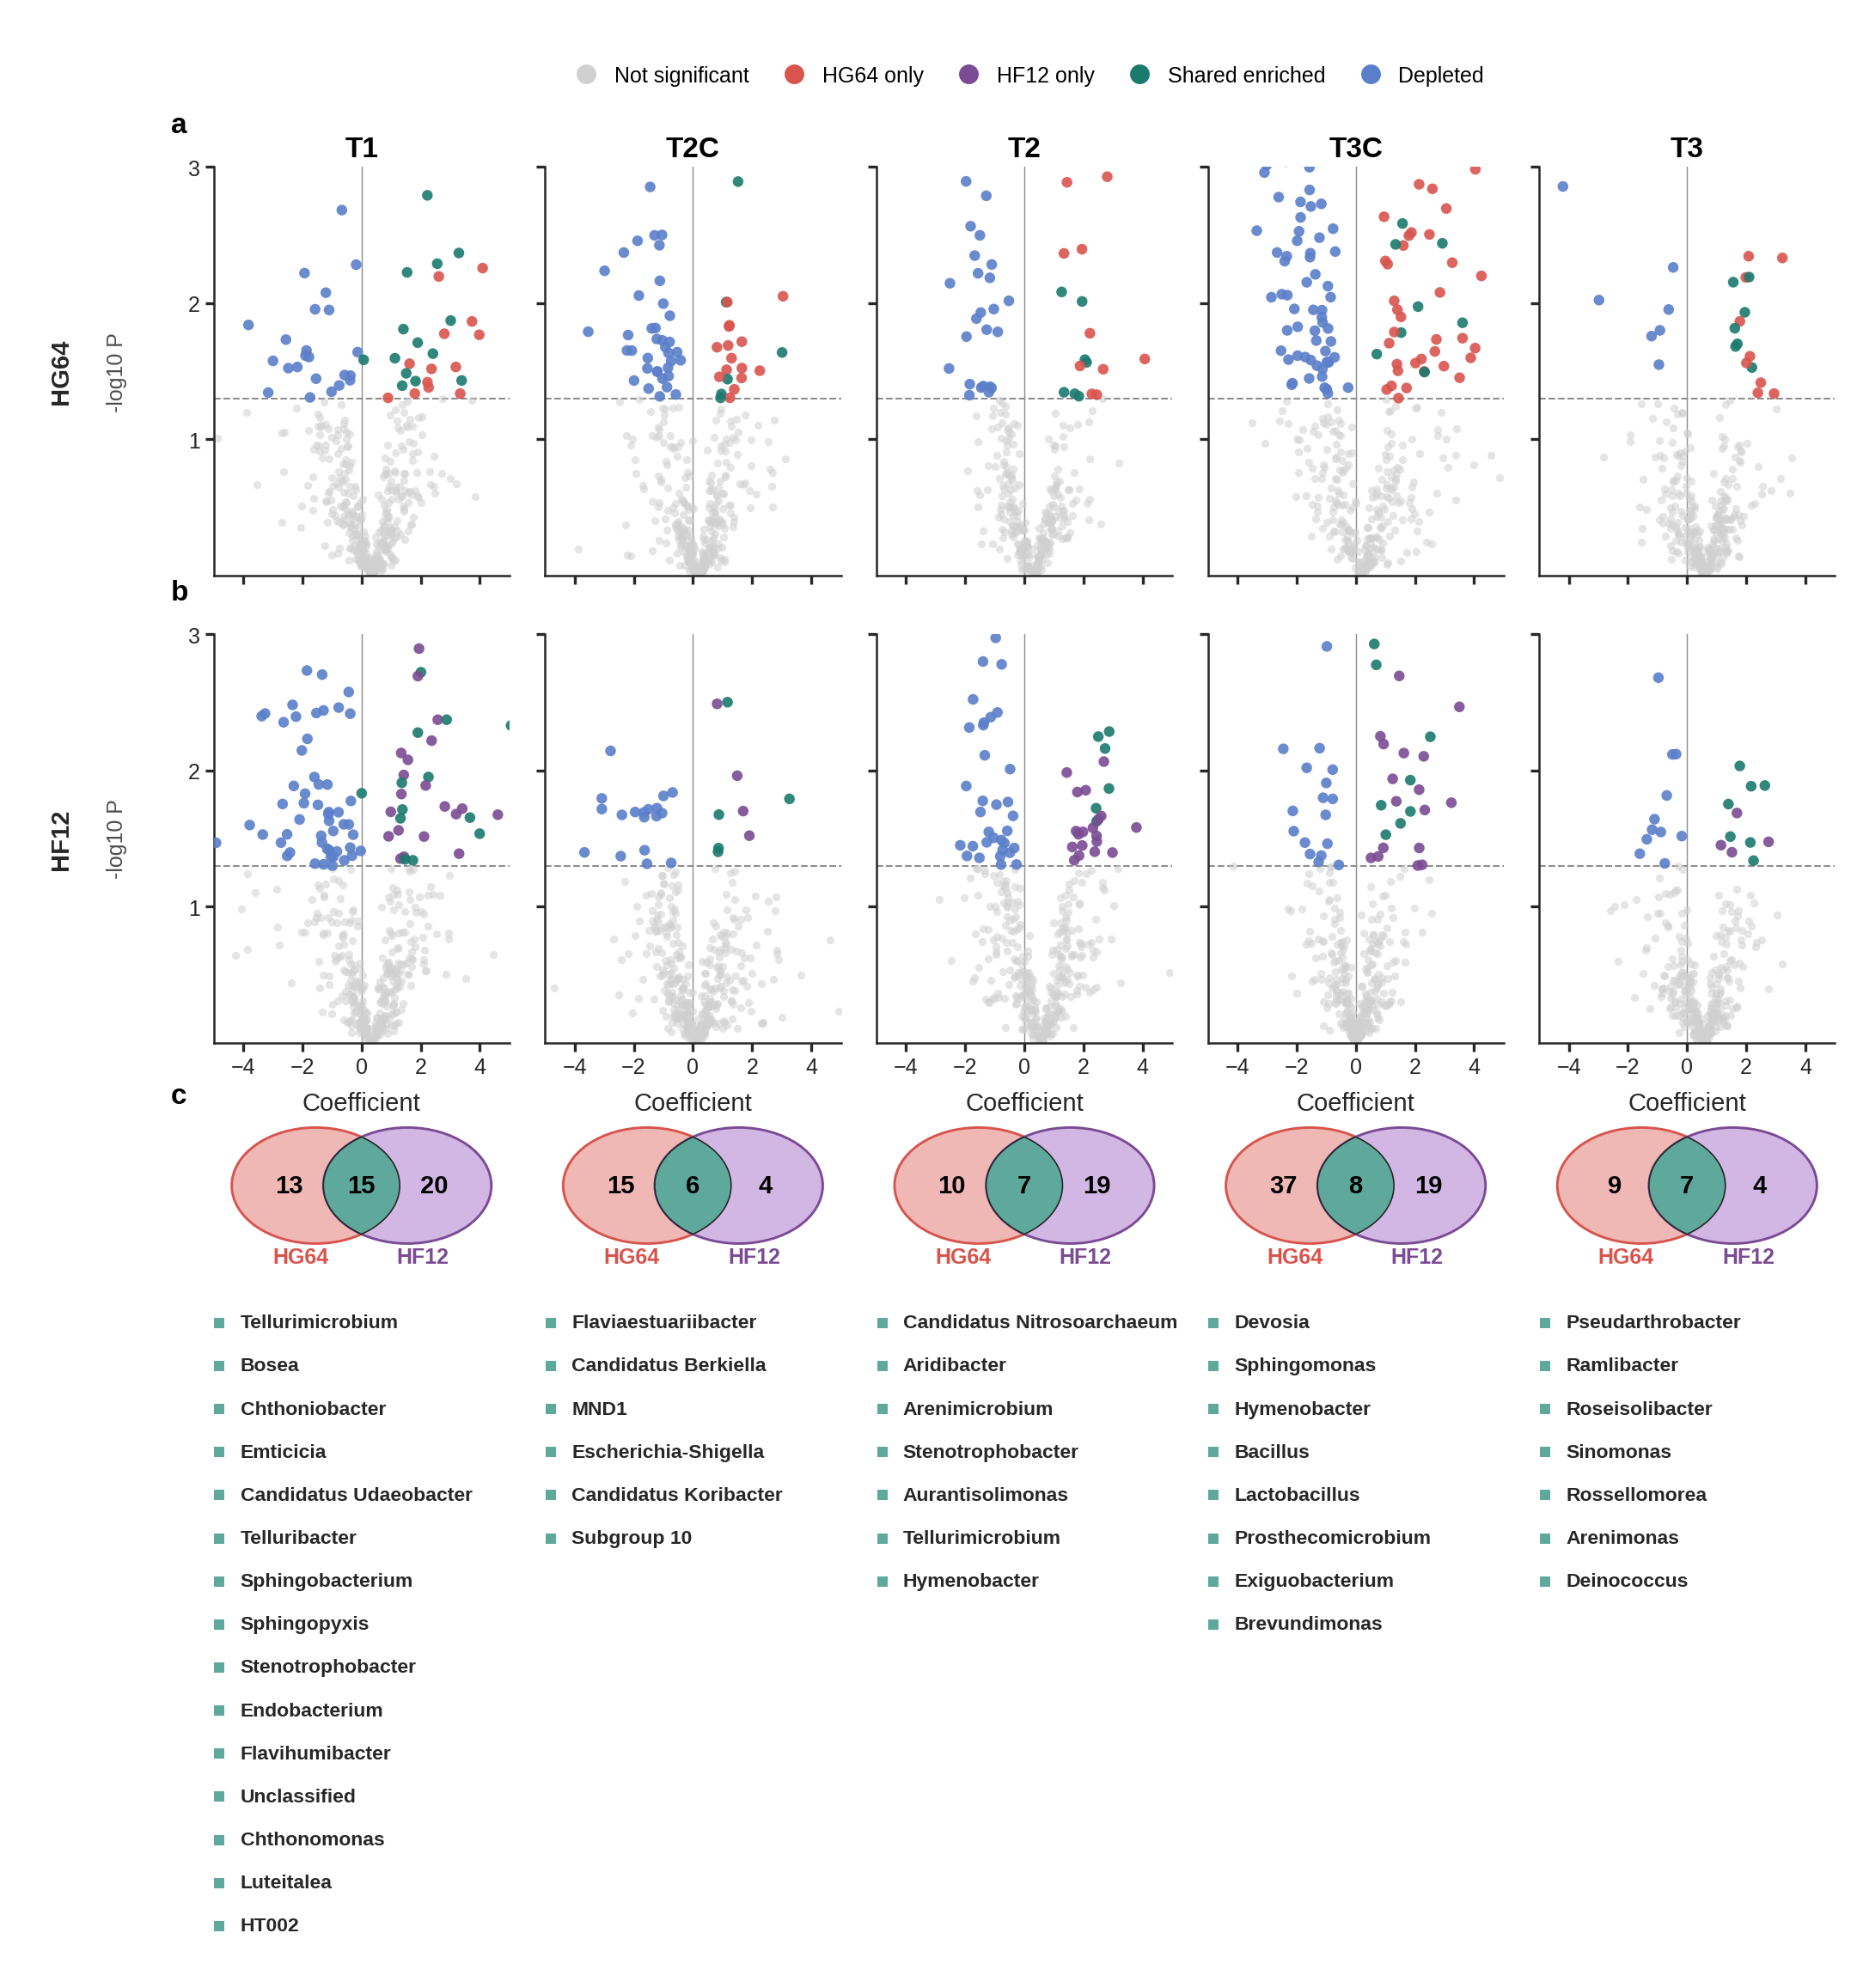
\includegraphics[width=0.94\linewidth]{Case-study-1-Fig2_16s_genus_enrichment.png}
\caption{Genus-level differential abundance in the 16S profiles of the resistant
  tomato parent HG64 and the resistant F1 hybrid HF12. (a,~b)~Volcano plots of
  MaAsLin~3 coefficients for HG64 (a) and HF12 (b) versus the pooled susceptible
  cultivars at each sampling condition. (c)~Overlap of genera with a positive
  coefficient and $P<0.05$ in both resistant cultivars.}
\label{fig:tomato-enrichment}
\end{figure}

\clearpage
\subsection{Additional evaluation details}
\label{app:evaluation}

The full Detailed, Medium, and Simple prompts used in the robustness evaluation
are reproduced below.

% Tighten list spacing without changing the 10 pt text size.
\renewenvironment{promptitems}{%
  \begin{itemize}%
  \setlength{\itemsep}{0pt}%
  \setlength{\parsep}{0pt}%
  \setlength{\topsep}{0.15em}%
  \setlength{\leftmargin}{1.2em}%
}{\end{itemize}}
\tcbset{before upper={\normalsize\setlength{\parskip}{0.15em}},
  title after break={Detailed prompt (continued)}}
\begin{promptbox}{Detailed prompt}
You are provided with rhizosphere shotgun metagenomic data and matched 16S rRNA
gene amplicon data from a tomato bacterial-wilt experiment. Conduct a
comprehensive exploratory and comparative microbiome analysis covering both 16S
rRNA and shotgun metagenomic profiling.
\prompthead{Data Characterization and Quality Control}
\begin{promptitems}
\item Describe all available metadata variables and the hierarchical structure
  of the dataset: cultivar genotype, resistance phenotype, sampling timepoint,
  inoculation treatment, biological replicate.
\item Visualize the experimental design, sequencing depth, and QC retention
  using sample-flow diagrams and distribution plots stratified by cultivar,
  timepoint, and treatment.
\end{promptitems}
\prompthead{16S rRNA Alpha Diversity Analysis}
\begin{promptitems}
\item Calculate Shannon diversity for each sample from the post-QC, non-chimeric
  ASV feature table after sequencing-depth normalization.
\item At each sampling timepoint, compare Shannon diversity among cultivars and
  between resistant and susceptible phenotype groups.
\item Visualize Shannon diversity with box/violin plots by cultivar and
  resistance phenotype, faceted by timepoint and treatment.
\end{promptitems}
\prompthead{16S rRNA Beta Diversity Analysis}
\begin{promptitems}
\item Quantify between-sample dissimilarity from the post-QC ASV feature table
  using \textbf{Weighted UniFrac}, \textbf{Unweighted UniFrac}, and
  \textbf{Bray--Curtis}.
\item Visualize weighted-UniFrac PCoA with samples colored by phenotype and
  shaped or faceted by cultivar, timepoint, and treatment.
\item Use PERMANOVA to assess resistance phenotype, cultivar, inoculation
  treatment, sampling timepoint, and prespecified interaction terms. Assess
  homogeneity of multivariate dispersion with PERMDISP before interpreting
  PERMANOVA.
\end{promptitems}
\prompthead{16S Taxonomic Profiling and Differential Abundance Analysis}
\begin{promptitems}
\item Conduct taxonomic classification and abundance-composition analysis.
\item At each independent sampling timepoint, identify taxa with significantly
  different abundances between each resistant focal cultivar and the susceptible
  control group.
\item Screen and summarize microbial markers significantly enriched in both
  resistant cultivars \textbf{HG64} and \textbf{HF12} at \textbf{T1},
  \textbf{T2C}, and \textbf{T2}. Define these shared taxa as core
  resistance-associated biomarkers.
\item Visualize composition with stacked bar plots and differential taxa with
  volcano plots or heatmaps; summarize shared biomarkers with an UpSet plot.
\end{promptitems}
\tcbbreak
\prompthead{Shotgun Metagenome Taxonomic and Differential Abundance Analysis}
\begin{promptitems}
\item Perform species-level taxonomic annotation and abundance profiling.
\item At each independent sampling timepoint, identify taxa with significantly
  different abundances between each resistant focal cultivar and the susceptible
  control group.
\item Screen and summarize markers significantly enriched in both \textbf{HG64}
  and \textbf{HF12} at \textbf{T1}, \textbf{T2C}, and \textbf{T2} as core
  resistance-associated biomarkers.
\item Visualize species-level composition with stacked bar plots and
  differential species with volcano plots or heatmaps; summarize shared markers
  with an UpSet plot.
\end{promptitems}
\end{promptbox}

\tcbset{title after break={Medium prompt (continued)}}
\begin{promptbox}{Medium prompt}
You are provided with rhizosphere shotgun metagenomic data and matched 16S rRNA
gene amplicon data from a tomato bacterial-wilt experiment. Conduct a
comprehensive exploratory and comparative microbiome analysis covering both 16S
rRNA and shotgun metagenomic profiling.
\prompthead{Data characterization}
\begin{promptitems}
\item Describe the dataset structure and assess quality.
\item Visualize experimental design, sequencing depth, and QC, stratified by
  cultivar, timepoint, and treatment.
\end{promptitems}
\prompthead{16S diversity, taxonomy, and differential abundance}
\begin{promptitems}
\item Compare alpha and beta diversity among cultivars and between resistant and
  susceptible groups, stratified by timepoint.
\item Profile taxonomic composition.
\item At each timepoint, identify taxa that differ between each resistant focal
  cultivar and the susceptible control.
\item Identify markers enriched in both \textbf{HG64} and \textbf{HF12} at
  \textbf{T1}, \textbf{T2C}, and \textbf{T2}.
\end{promptitems}
\prompthead{Shotgun taxonomy and differential abundance}
\begin{promptitems}
\item Profile species-level composition.
\item At each timepoint, identify species that differ between each resistant
  focal cultivar and the susceptible control.
\item Identify markers enriched in both \textbf{HG64} and \textbf{HF12} at
  \textbf{T1}, \textbf{T2C}, and \textbf{T2}.
\end{promptitems}
\end{promptbox}

\tcbset{title after break={Simple prompt (continued)}}
\begin{promptbox}{Simple prompt}
You are provided with rhizosphere shotgun metagenomic data and matched 16S rRNA
gene amplicon data from a tomato bacterial-wilt experiment. Analyze the dataset
and identify microbiome patterns associated with wilt resistance, using both 16S
and shotgun profiles.
\end{promptbox}

% Keep the comparison methods and their two supporting tables together.
\clearpage
Analytical outputs were averaged across completed replicate sessions and aligned
on shared entries before comparison. Diversity comparisons included per-sample
Shannon indices ($n = 60$) and pairwise weighted UniFrac distances ($n =
1{,}770$). Taxonomic abundance comparisons used shared sample--taxon entries
with a session-mean relative abundance of at least 5\% in every compared group.
This filter limited the influence of fluctuations in rare taxa on rank-based
comparisons. Differential-abundance comparisons included all shared taxa without
an abundance threshold and were restricted to sessions using identical
statistical software (Tables~\ref{tab:da-model-methods}
and~\ref{tab:da-prompt-methods}; Figure~\ref{fig:robustness-prompts}).

\begin{table}[H]
\centering
\caption{Replicate sessions and shared entries for cross-model DESeq2
  comparisons.}
\label{tab:da-model-methods}
\normalsize
\setlength{\tabcolsep}{5pt}
\renewcommand{\arraystretch}{1.12}
\begin{tabularx}{\linewidth}{@{}>{\raggedright\arraybackslash}Xlcccc@{}}
\toprule
Dataset & Prompt
  & \shortstack{DeepSeek\\Pro}
  & \shortstack{DeepSeek\\Flash}
  & \shortstack{GLM\\Flash}
  & \shortstack{Shared\\entries} \\
\midrule
16S rRNA gene, genus & Detailed & 1/3 & 2/3 & 3/3 & 1,724 \\
16S rRNA gene, genus & Medium & 1/3 & 2/3 & 1/3 & 2,659 \\
Shotgun metagenome, species & Detailed & 1/3 & 2/3 & 2/3 & 228 \\
\bottomrule
\end{tabularx}
\par\vspace{0.4em}
{\normalsize Values for each model indicate the number of independent replicates
  (out of three) that selected DESeq2. Shared entries are the taxa evaluated
  across all three models. Shotgun results under the medium prompt were not
  compared because no single differential-abundance method was selected by all
  three models.}
\end{table}

\begin{table}[H]
\centering
\caption{Replicate sessions and shared entries for prompt-level
  differential-abundance comparisons.}
\label{tab:da-prompt-methods}
\normalsize
\setlength{\tabcolsep}{6pt}
\renewcommand{\arraystretch}{1.12}
\begin{tabular}{@{}llccc@{}}
\toprule
Model & Method
  & \shortstack{Detailed\\sessions}
  & \shortstack{Medium\\sessions}
  & \shortstack{Shared\\entries} \\
\midrule
\multicolumn{5}{@{}l}{\textit{16S rRNA gene, genus}} \\
\addlinespace
\texttt{deepseek-v4-pro} & DESeq2 & 1/3 & 1/3 & 891 \\
\texttt{deepseek-v4-flash} & DESeq2 & 2/3 & 2/3 & 5,108 \\
\texttt{glm5.3-flash} & DESeq2 & 3/3 & 1/3 & 3,984 \\
\addlinespace
\multicolumn{5}{@{}l}{\textit{Shotgun metagenome, species}} \\
\addlinespace
\texttt{deepseek-v4-pro} & Wilcoxon & 1/3 & 1/3 & 39 \\
\texttt{deepseek-v4-flash} & Mann--Whitney $U$ & 1/3 & 1/3 & 120 \\
\texttt{glm5.3-flash} & DESeq2 & 2/3 & 1/3 & 52 \\
\bottomrule
\end{tabular}
\par\vspace{0.4em}
{\normalsize Session counts indicate the number of independent replicates (out
  of three) that selected the specified statistical method under each prompt
  level. Shared entries are the taxa evaluated across both prompt levels.}
\end{table}

% Keep this comparison figure before the execution-ablation material.
\clearpage
\begin{figure}[H]
\centering
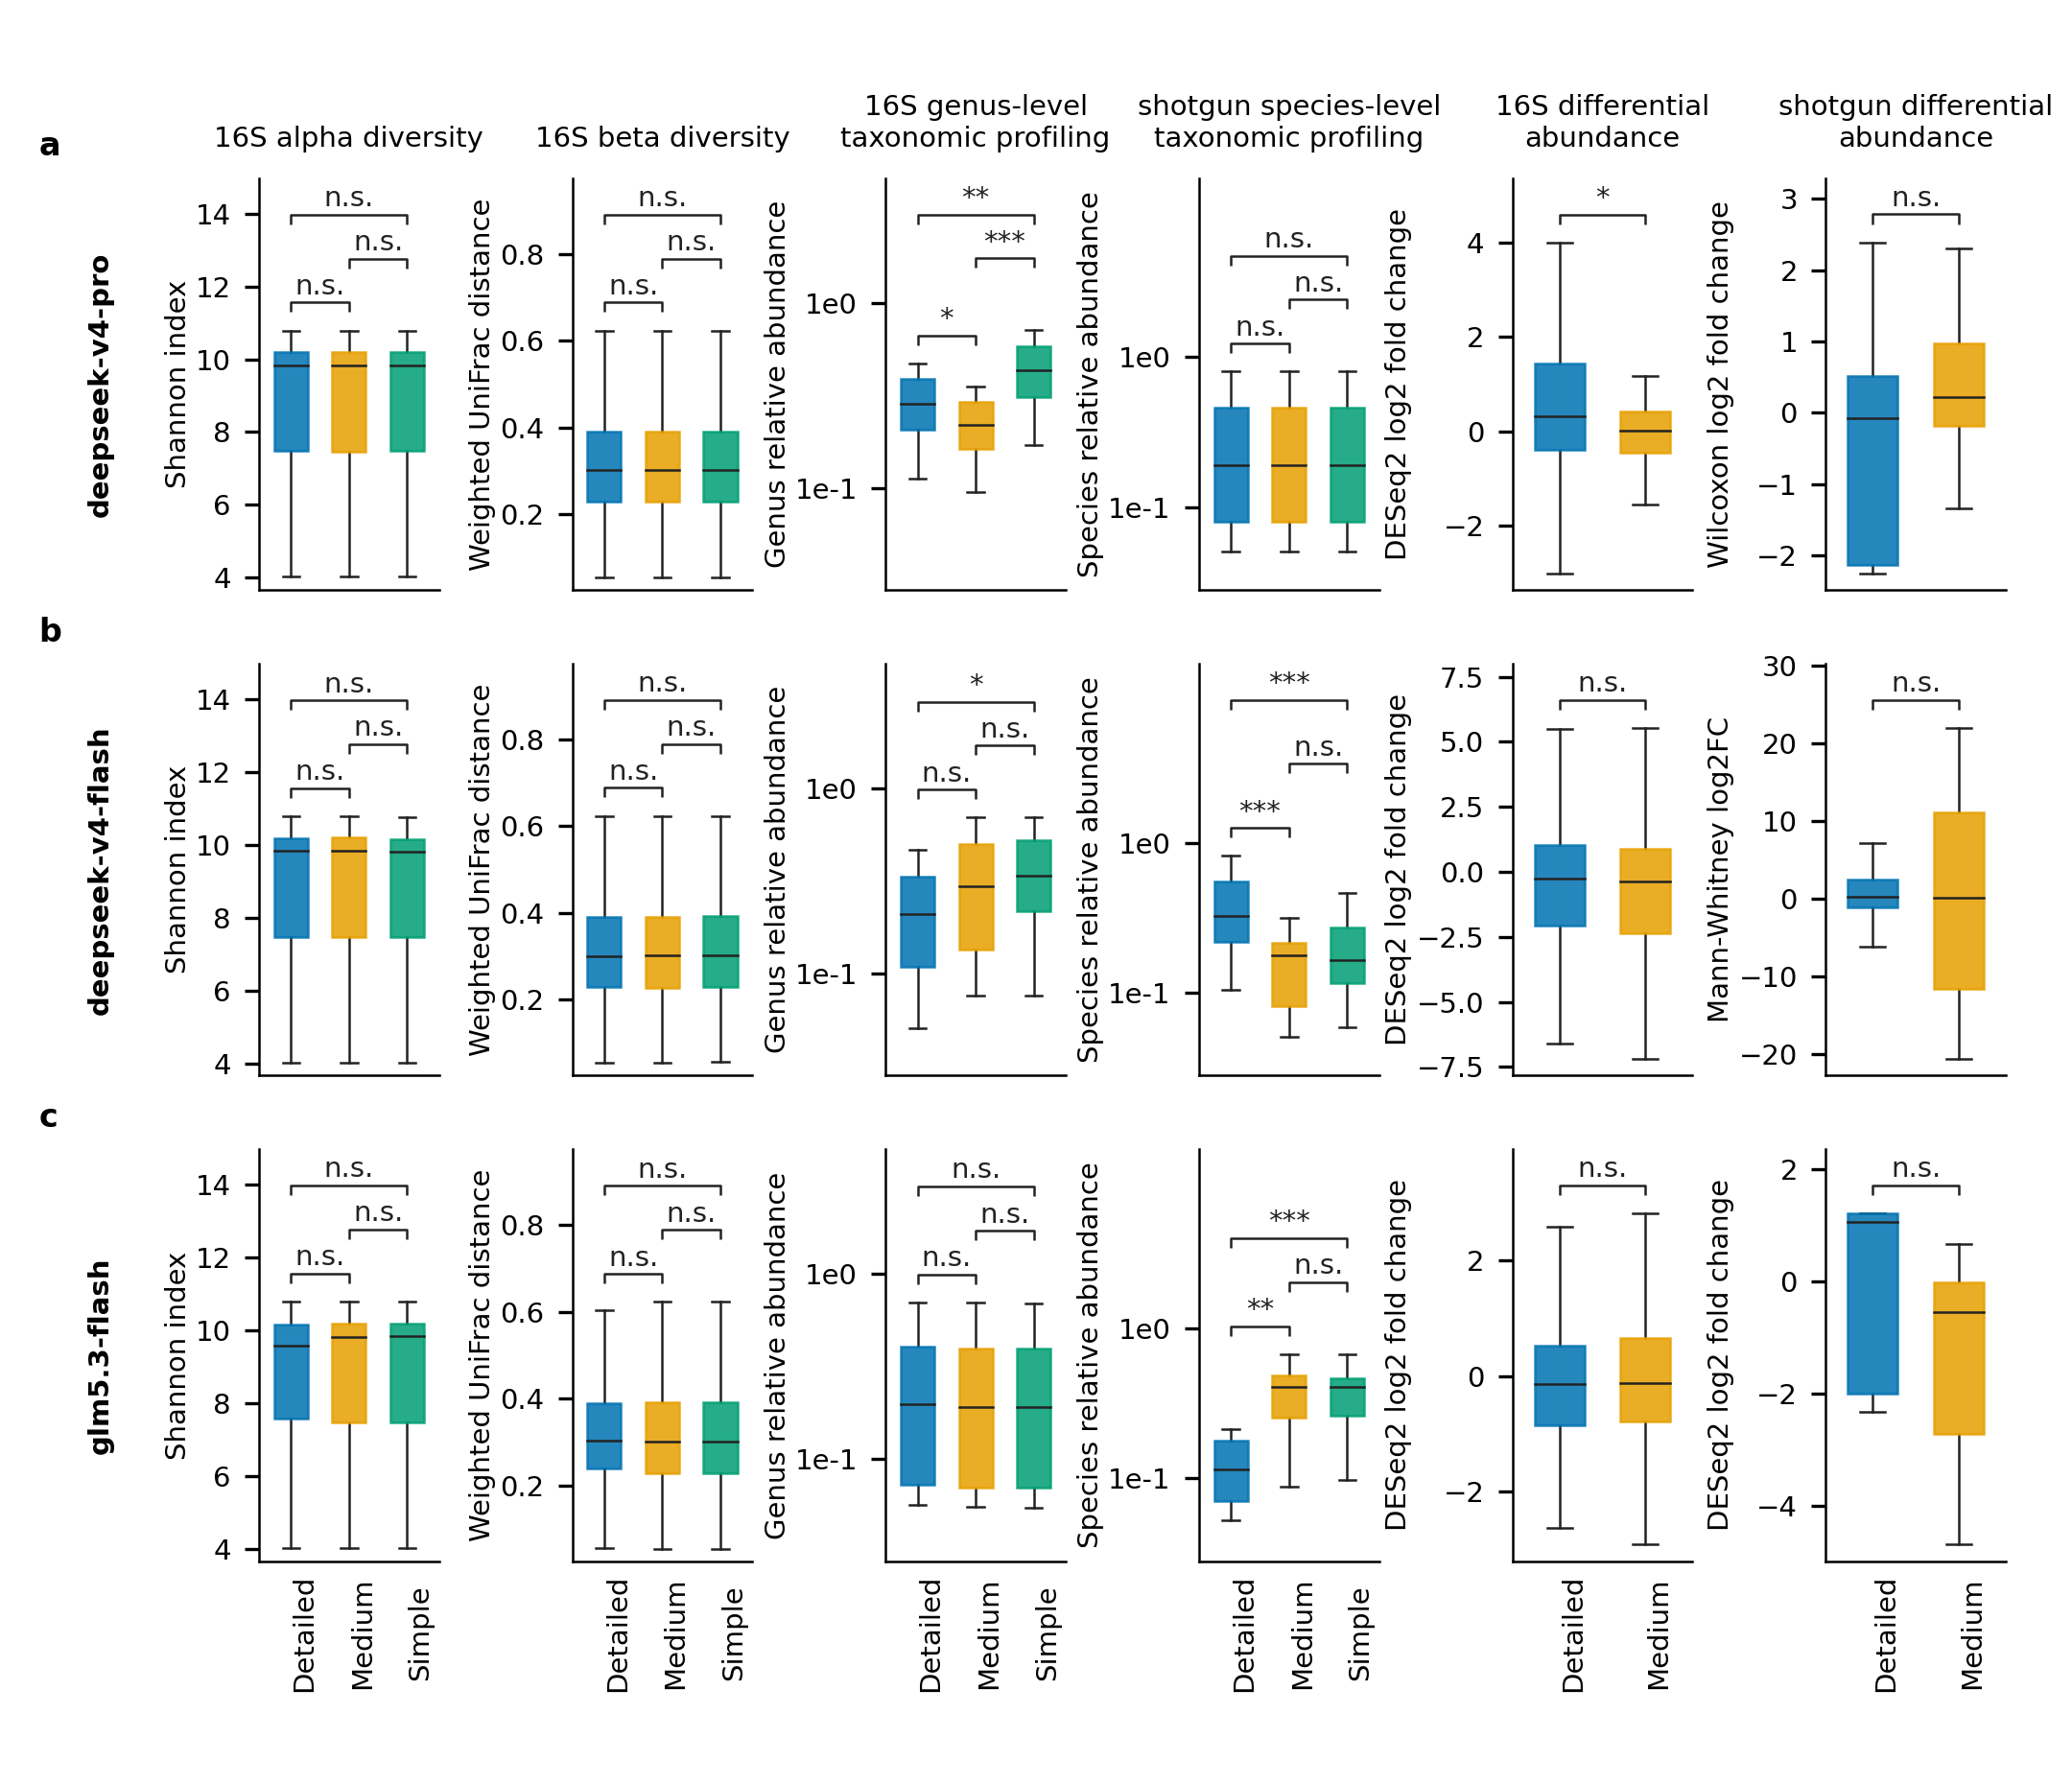
\includegraphics[width=0.92\linewidth]{by_prompt_models.png}
\caption{Comparison of analytical outputs across prompt levels within each
  model. Rows represent \texttt{deepseek-v4-pro}, \texttt{deepseek-v4-flash},
  and \texttt{glm5.3-flash}. The first four columns display 16S Shannon
  diversity indices, pairwise weighted UniFrac distances, 16S genus-level
  relative abundances, and shotgun species-level relative abundances across
  prompt levels. The remaining two columns compare differential-abundance
  $\log_2$ fold changes between the detailed and medium prompts (16S: DESeq2;
  shotgun: the test shared within each model,
  Table~\ref{tab:da-prompt-methods}). Brackets in the first four columns
  indicate two-sided Mann--Whitney $U$ tests with Holm correction across the
  three prompt pairs within each model; brackets in the differential-abundance
  panels indicate comparisons between the detailed and medium prompts. *$P <
  0.05$; **$P < 0.01$; ***$P < 0.001$; n.s., adjusted $P \ge 0.05$. Values are
  derived from repeated analyses of the same Case~1 dataset and do not represent
  independent biological replicates.}
\label{fig:robustness-prompts}
\end{figure}

% Keep the ablation description and its table on the same page.
\clearpage
Table~\ref{tab:ablation-replicates} provides per-session outputs, method
adherence, model and tool calls, and token consumption for the execution
ablation.

\begin{table}[H]
\centering
\caption{Per-session outputs, method adherence, tool calls, and token
  consumption in the execution ablation.}
\label{tab:ablation-replicates}
\normalsize
\setlength{\tabcolsep}{4pt}
\renewcommand{\arraystretch}{1.12}
\textbf{(a) Outputs, method adherence, and model calls}\par\smallskip
\begin{tabular*}{\linewidth}{@{\extracolsep{\fill}}llccc@{}}
\toprule
Condition & Session
  & \shortstack{Outputs\\(of 9)}
  & \shortstack{Methods\\(of 8)}
  & \shortstack{Model\\calls} \\
\midrule
\texttt{full} & 1 & 9/9 & 8/8 & 150 \\
\texttt{full} & 2 & 9/9 & 8/8 & 124 \\
\texttt{full} & 3 & 9/9 & 8/8 & 126 \\
\texttt{full} & Mean / sum & 27/27 & 24/24 & 133.3 \\
\addlinespace
\texttt{no-patch} & 1 & 8/9 & 8/8 & 211 \\
\texttt{no-patch} & 2 & 9/9 & 8/8 & 403 \\
\texttt{no-patch} & 3 & 9/9 & 8/8 & 245 \\
\texttt{no-patch} & Mean / sum & 26/27 & 24/24 & 286.3 \\
\bottomrule
\end{tabular*}
\par\medskip
\textbf{(b) Tool calls and token consumption}\par\smallskip
\begin{tabular*}{\linewidth}{@{\extracolsep{\fill}}llcccc@{}}
\toprule
Condition & Session
  & \texttt{exec}
  & \shortstack{\texttt{process}}
  & \shortstack{\texttt{yield}}
  & \shortstack{Tokens\\($\times 10^6$)} \\
\midrule
\texttt{full} & 1 & 91 & 1 & 17 & 12.92 \\
\texttt{full} & 2 & 74 & 21 & 5 & 14.81 \\
\texttt{full} & 3 & 82 & 0 & 13 & 15.84 \\
\texttt{full} & Mean / sum & 82.3 & 7.3 & 11.7 & 14.53 \\
\addlinespace
\texttt{no-patch} & 1 & 77 & 102 & 0 & 23.77 \\
\texttt{no-patch} & 2 & 142 & 227 & 0 & 49.32 \\
\texttt{no-patch} & 3 & 99 & 136 & 0 & 32.15 \\
\texttt{no-patch} & Mean / sum & 106.0 & 155.0 & 0.0 & 35.08 \\
\bottomrule
\end{tabular*}
\par\vspace{0.4em}
{\normalsize Summary rows pool outputs and method requirements across the three
  sessions. Tool-call counts and token consumption in those rows are per-session
  means. Total tokens are input plus output tokens, including reasoning tokens.}
\end{table}
